\chapter{Analisis}
\label{chap:analisis}

Pada bab ini dijelaskan mengenai analisis grafik dari data sensor-sensor pada \textit{smartphone} ketika sedang mengangguk dan menggeleng, analisis aplikasi-aplikasi sejenis, dan analisis metode pendeteksian gerakan kepala. 

\section{Analisis Aplikasi Sejenis}
\label{sec:analisis_aplikasi_sejenis}

Pada saat skripsi ini dibuat, aplikasi sejenis pada perangkat VR Google Cardboard hanya ada satu aplikasi saja. Aplikasi tersebut adalah aplikasi InMind VR. Aplikasi sejenis pada perangkat VR Oculust Rift adalah Trial of the Rift Drifter dengan Asunder yang dikembangkan oleh AldinDynamics \cite{aldin_dynamics}. Aplikasi sejenis pada VR Oculust Rift tidak dapat dianalisis karena penulis tidak memiliki perangkat Oculust Rift. \\

\textbf{Analisis InMind VR}\\

InMind VR merupakan permainan VR yang seolah-olah pengguna berada dalam sel-sel otak seorang manusia. Permainan ini dimainkan dengan mengarahkan arah pandang kepala ke arah sel-sel neuron yang dapat menyebabkan gangguan mental (Gambar \ref{fig:screenshot_inmind_task}). Ada 50 sel neuron yang dapat menyebabkan gangguan mental. Sel-sel yang dapat menyebabkan gangguan mental adalah sel-sel yang berwarna merah seperti pada Gambar \ref{fig:screenshot_inmind_gameplay}.

\begin{figure}[htbp]
\centering
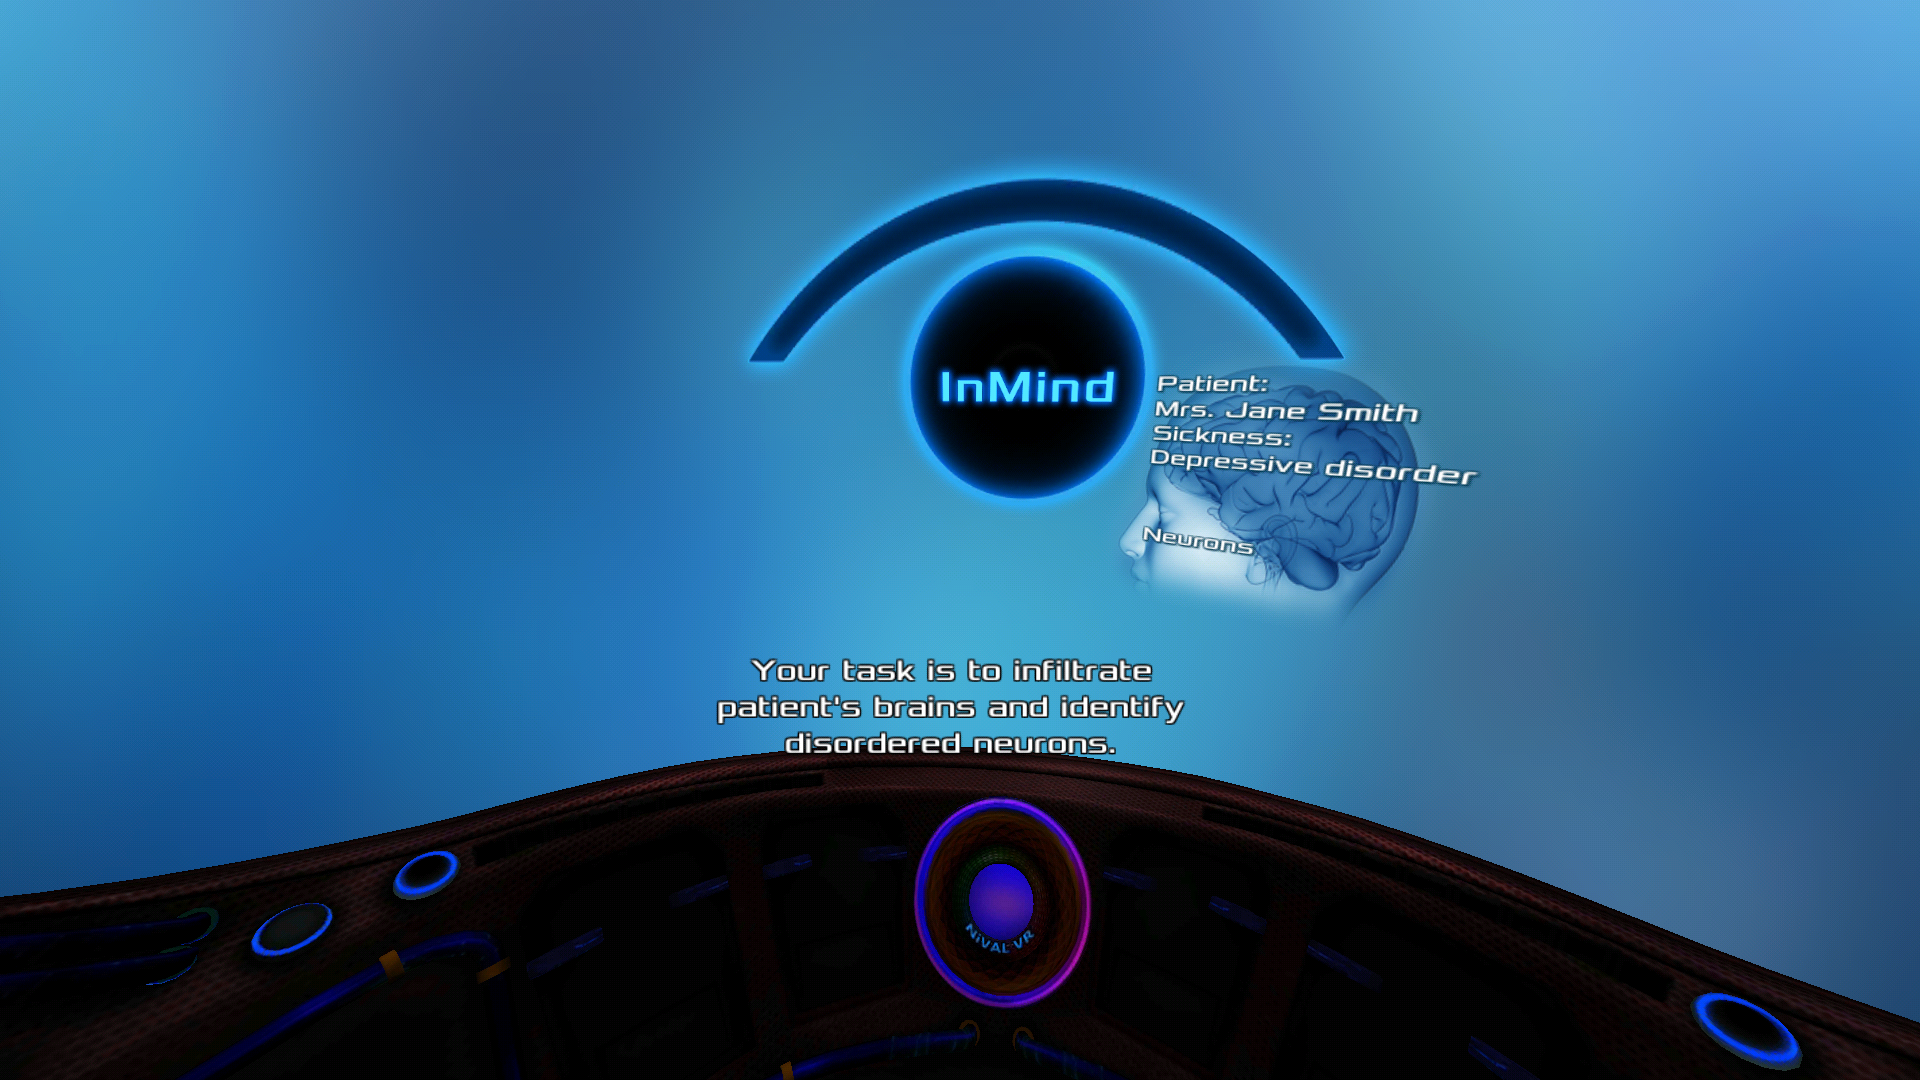
\includegraphics[scale=0.6]{Gambar/screenshot-inmind-task.png}
\caption{\textit{Screenshot} task yang diberikan aplikasi InMind VR.}
\label{fig:screenshot_inmind_task}
\end{figure}

Pada permulaan permainan pengguna diberi pertanyaan apakah pengguna sudah siap untuk melakukan permainan tersebut seperti yang ditunjukkan pada Gambar \ref{fig:screenshot_inmind_nod}.

\begin{figure}[htbp]
\centering
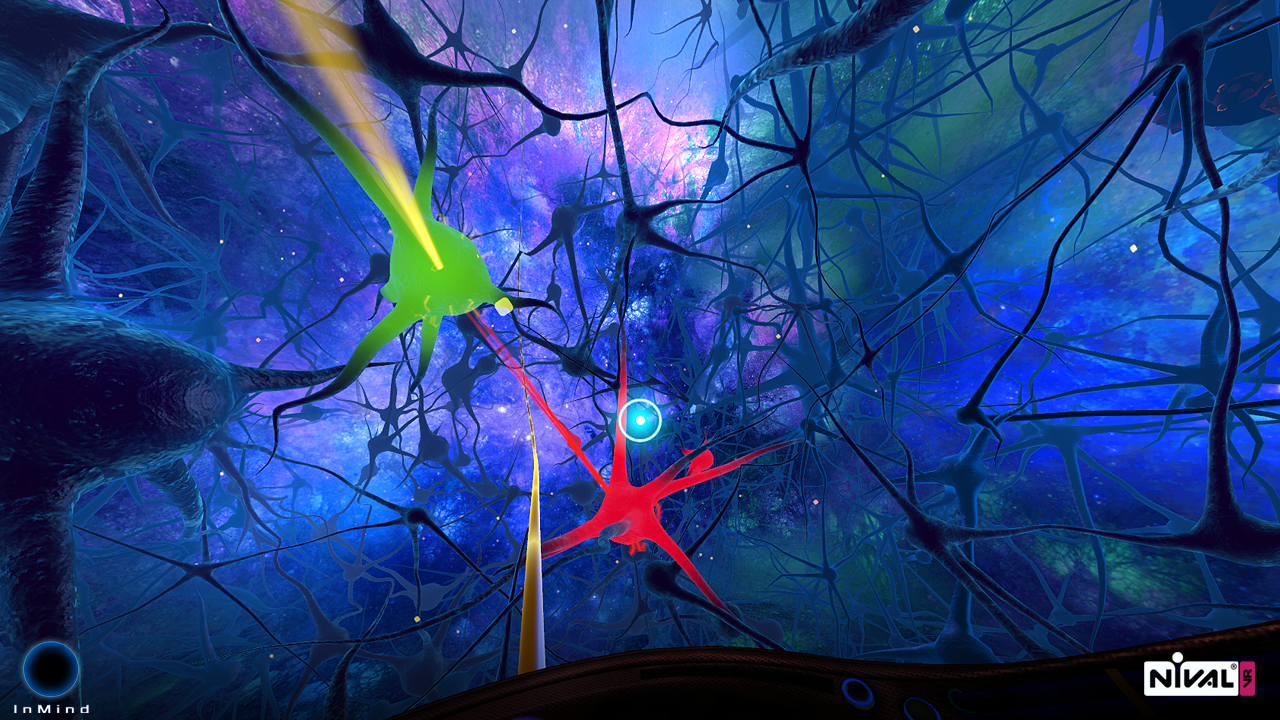
\includegraphics[scale=0.7]{Gambar/screenshot-inmind-gameplay.jpg}
\caption{\textit{Screenshot} aplikasi InMind VR ketika permainan berlangsung.}
\label{fig:screenshot_inmind_gameplay}
\end{figure}

Analisis dilakukan dengan cara mengetes aplikasi ini dengan mengangguk dan menggeleng yang spesifik. Mengangguk dilakukan dengan cara-cara berikut:
\begin{enumerate}
	\item Mengangguk secara pelan.
	\item Mengangguk yang diawali dengan gerakan ke atas.
	\item Melihat kebawah saja tanpa membalikkan kepala ke posisi semula.
	\item Tidak menggerakkan kepala sama sekali.
\end{enumerate}

Keempat percobaan tersebut memiliki tujuan masing-masing. Percobaan pertama dilakukan untuk apakah gerakan secara perlahan diartikan sebagai gerakan mengangguk atau tidak. Percobaan kedua dilakukan untuk mengetahui apakah gerakan anggukan dengan gerakan keatas terlebih dahulu dianggap mengangguk atau tidak. Percobaan ketiga dilakukan untuk mengetahui apakah gerakan melihat kebawah dianggap mengangguk atau tidak. Percobaan keempat dilakukan untuk mengetahui respon dari aplikasi jika pengguna tidak melakukan gerakan anggukkan atau tidak. 

Dari keempat percobaan mengangguk yang dilakukan, hanya percobaan pertama dengan percobaan ketiga yang terdeteksi mengangguk. Dapat disimpulkan dengan hanya menggerakkan kepala ke bawah saja sudah dapat dianggap mengangguk oleh aplikasi ini. Pada percobaan kedua dan keempat terjadi keganjilan dari pendeteksian anggukan. Pada percobaan kedua dan keempat aplikasi tetap melanjutkan permainan setelah beberapa detik berlalu. Sel-sel yang dapat menyebabkan gangguan mental adalah sel-sel yang berwarna merah seperti pada Gambar \ref{fig:screenshot_inmind_gameplay}. 

Ketika dilakukan percobaan menggeleng, tidak ada respons apa pun dari aplikasi ini. Aplikasi ini tetap melanjutkan ke permainan setelah beberapa detik telah berlalu. Hal tersebut menyimpulkan bahwa aplikasi ini tidak dapat mendeteksi gerakan menggeleng. Oleh karena itu hal yang dilakukan oleh aplikasi ini hanyalah melihat apakah pengguna sudah melihat ke bawah atau belum saja.

\begin{figure}[htbp]
\centering
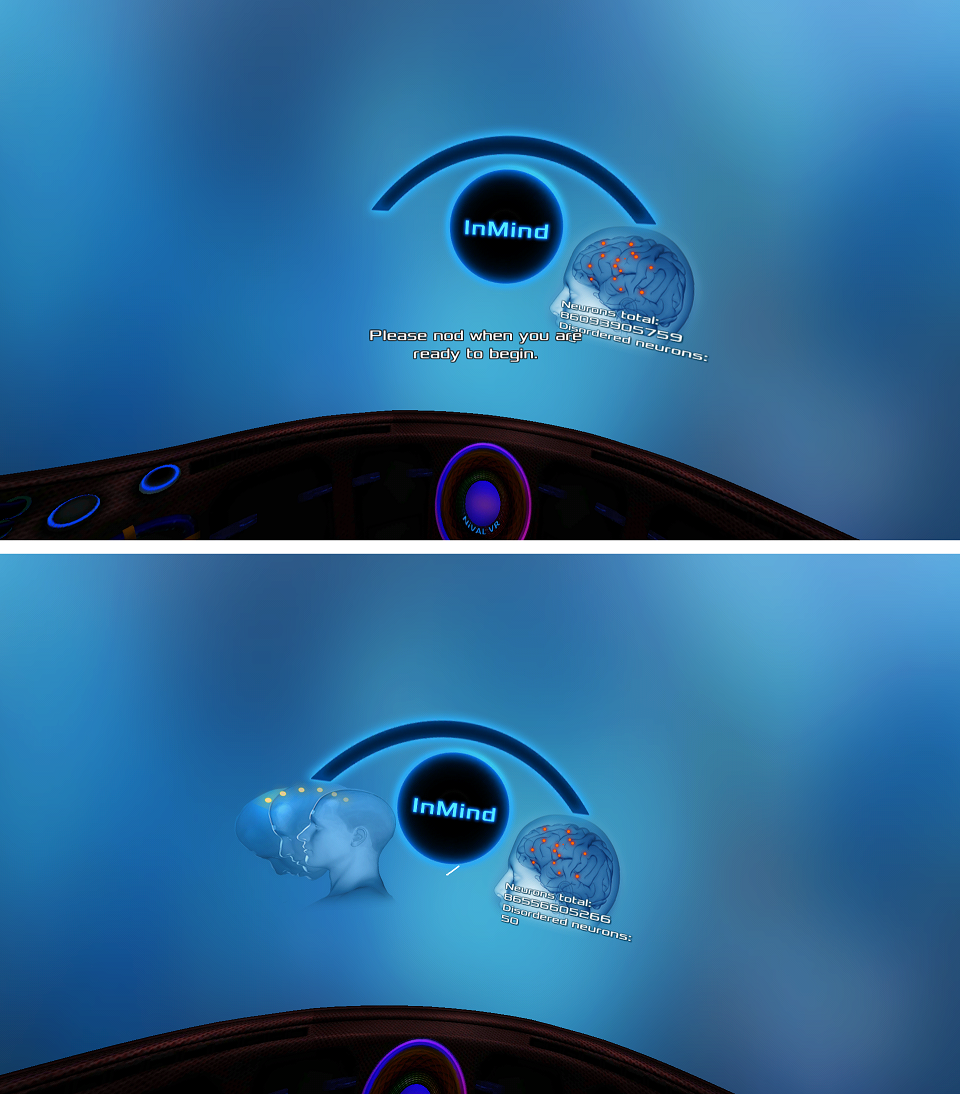
\includegraphics[scale=0.6]{Gambar/screenshot-inmind-nod.png}
\caption{\textit{Screenshot} aplikasi InMind VR ketika meminta pengguna untuk mengangguk jika telah siap.}
\label{fig:screenshot_inmind_nod}
\end{figure}



\section{Perekaman Data Sensor}
\label{sec:perekaman_data_sensor}

Pada analisis ini dilakukan perekaman mengangguk dan menggeleng dengan sensor-sensor pada Android. Perekaman-perekaman ini dilakukan pada tiga kondisi muka pengguna. Kondisi muka yang pertama adalah kondisi muka pengguna ketika menghadap ke depan, digambarkan dengan Gambar \ref{fig:posisi-muka} bagian (a). Kondisi muka yang kedua adalah kondisi muka pengguna ketika menghadap ke atas sekitar $45^{\circ}$ dari pandangan muka menghadap ke atas digambarkan dengan Gambar \ref{fig:posisi-muka} bagian (b). Kondisi muka yang ketiga adalah kondisi muka ketika menghadap serong ke kiri atas digambarkan dengan Gambar \ref{fig:posisi-muka} bagian (c). Anggukan yang dilakukan oleh pengguna hanya sebanyak satu kali mengangguk ke bawah saja. Sedangkan dalam menggeleng bergerak ke kiri terlebih dahulu dan ke kanan setelahnya dan diakhiri pada posisi muka kembali ke posisi awal. Perekaman grafik hanya akan dilakukan satu kali saja untuk setiap posisi. Setiap posisi akan dilakukan gerakan mengangguk dan menggeleng masing-masing satu kali.

\begin{figure}[htbp]
\centering
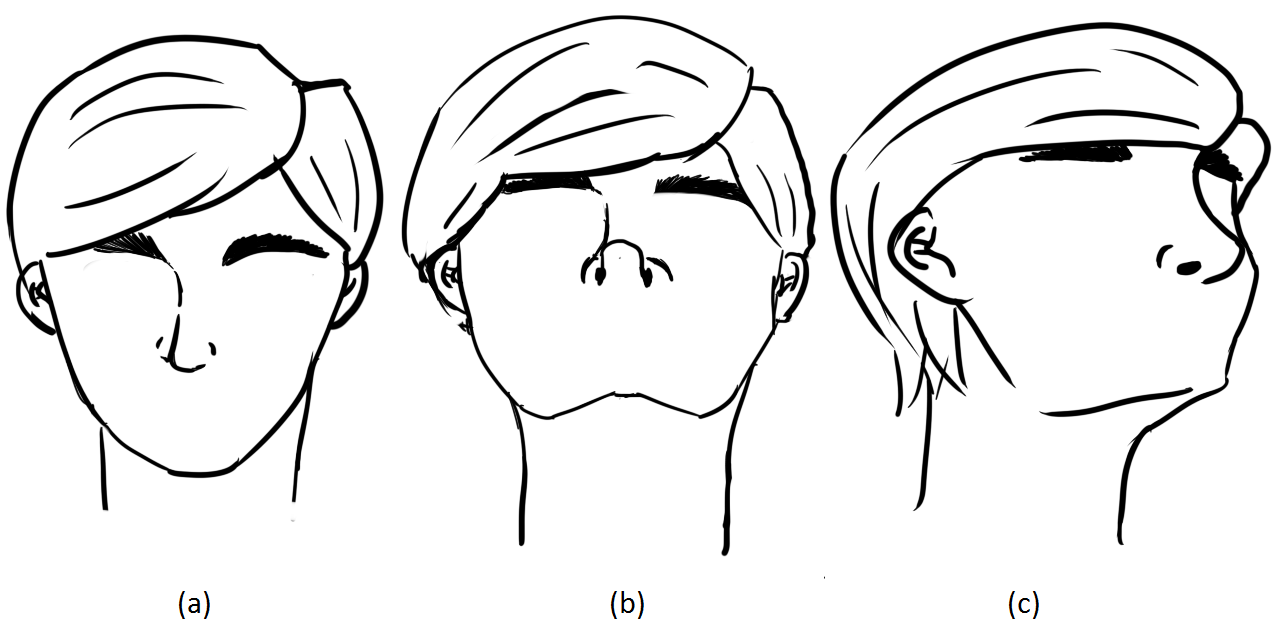
\includegraphics[scale=0.4]{Gambar/posisi-muka.png}
\caption{Gambar untuk mendeskripsikan posisi dari muka sebelum melakukan gerakan menggeleng atau mengangguk. Gambar (a) adalah kondisi muka ketika sedang menghadap ke depan. Gambar (b) adalah kondisi muka ketika sedang menghadap ke atas. Gambar(c) adalah kondisi muka ketika sedang menghadap ke serong kiri atas.}
\label{fig:posisi-muka}
\end{figure}

Grafik-grafik yang ditunjukkan pada bab ini memiliki beberapa karakteristik. Sumbu y pada grafik menunjukkan representasi besar nilainya, sedangkan sumbu x menunjukkan representasi waktunya. Grafik yang ditunjukkan memiliki beberapa nilai, tergantung dari jumlah nilai yang dikembalikan untuk setiap sensornya. Contohnya pada sensor \textit{accelerometer} yang memiliki tiga jenis nilai, pada grafik terbentuk tiga buah garis nilai. Aplikasi merekam beberapa sensor secara langsung ketika pengguna mengangguk atau menggeleng, sehingga nilai waktunya sama untuk kondisi muka yang sama walaupun sensornya berbeda.

Analisis grafik data sensor-sensor pada Android dilakukan dengan membuat suatu aplikasi perekam sensor-sensor yang ada pada \textit{smartphone} Android terlebih dahulu. Aplikasi ini merekam nilai-nilai yang dihasilkan dari sebagian sensor-sensor pada android setiap ada perubahan. Pada skripsi ini, nilai sensor-sensor yang dibutuhkan adalah sensor-sensor yang merupakan sensor pendeteksi gerak. Seperti yang sudah dijelaskan subbab \ref{sec:android_sensor_framework}, sensor gerak meliputi \textit{accelerometer}, sensor gravitasi, \textit{gyroscope}, dan \textit{rotation vector}. Karena sensor gravitasi merupakan sensor \textit{accelerometer} yang dikembangkan sehingga tidak digunakan pada analisis grafik sensor ini. Sehingga sensor-sensor yang digunakan untuk dianalisis adalah sensor \textit{accelerometer}, \textit{gyroscope}, dan \textit{rotation vector}. Aplikasi menyimpan nilai sensor-sensor menggunakan format CSV \textit{(Comma Separated Values)}. Dari data yang diperoleh oleh aplikasi tersebut dibuat grafik-nya menggunakan aplikasi Microsoft Excel. Penjelasan dari setiap grafik dijelaskan pada subbab \ref{sec:analisis_grafik_sensor_accelerometer} hingga subbab \ref{sec:analisis_grafik_sensor_rotation_vector}.

\subsection{Perekaman Grafik Sensor \textit{Accelerometer}}
\label{sec:analisis_grafik_sensor_accelerometer}

Seperti yang sudah dijelaskan pada bab sebelumnya, sensor \textit{accelerometer} mendeteksi seluruh percepatan yang terjadi pada perangkat Android. Pada perekaman ini, perangkat Android diletakkan di depan muka pengguna, sehingga percepatan yang memengaruhi perangkat Android hanya percepatan gravitasi dengan percepatan yang dilakukan oleh gerakan kepala pengguna. 

\begin{figure}[htbp]
\centering
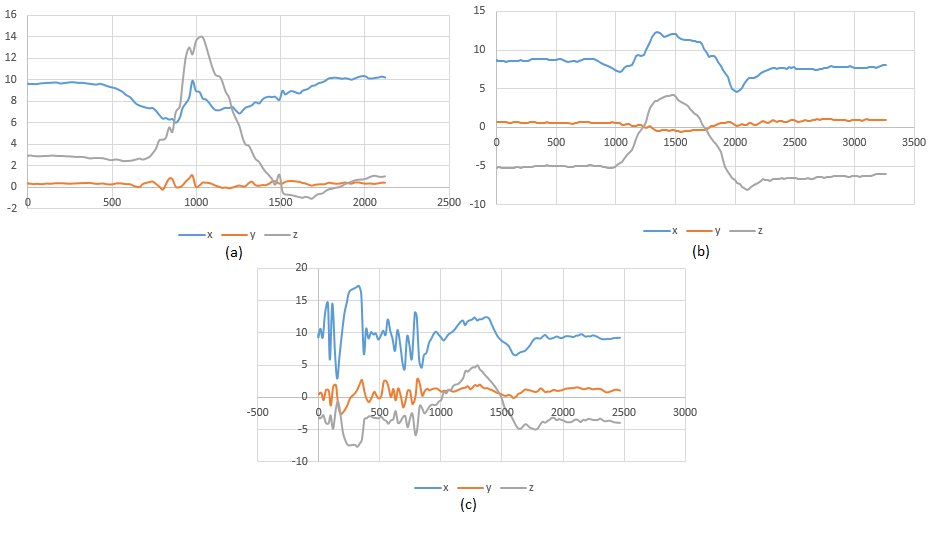
\includegraphics[scale=0.6]{Gambar/grafik-sensor-accelerometer-mengangguk.png}
\caption{Grafik nilai kuaternion dari sensor \textit{accelerometer} ketika pengguna mengangguk dengan posisi muka awal (a) menghadap ke depan, (b) menghadap ke atas, (c) menghadap ke kiri atas.} 
\label{fig:grafik-sensor-accelerometer-mengangguk}
\end{figure}

Gambar \ref{fig:grafik-sensor-accelerometer-mengangguk} merupakan grafik-grafik yang terbentuk dari nilai yang diterima oleh sensor \textit{accelerometer} ketika pengguna sedang mengangguk. Pada Gambar \ref{fig:grafik-sensor-accelerometer-mengangguk} grafik (a) terlihat nilai z menaik dan nilai x menurun ketika sedang mengangguk. Tetapi nilai x kembali menaik ketika nilai z sudah hampir mencapai nilai tertinggi. Sedangkan nilai y terlihat cukup konstan di sekitar angka 0. Pada grafik (b) terlihat nilai x dengan y memiliki pola yang serupa ketika mengangguk. Kedua nilai menaik ketika pengguna sedang mengangguk. Nilai x berada pada nilai sekitar sebesar 9 sedangkan nilai z bernilai sekitar sebesar -5. Sama seperti pada grafik (a) nilai y terlihat konstan di sekitar angka 0. Selanjutnya grafik (c) pada Gambar \ref{fig:grafik-sensor-accelerometer-mengangguk} merupakan grafik yang terbentuk dari nilai yang diterima oleh sensor \textit{accelerometer} ketika pengguna mengangguk dan sedang menghadap ke kiri atas. Grafik pada bagian ini sangat tidak beraturan. Pada Grafik ini sulit untuk membedakan kondisi kapan pengguna sedang mengangguk. Goncangan yang terjadi terhadap \textit{smartphone}, seperti munculnya notifikasi mungkin dapat menyebabkan hal ini. Namun pada waktu mencapai 1000 milidetik terlihat cukup stabil. Pada grafik (c) di Gambar \ref{fig:grafik-sensor-accelerometer-mengangguk} juga menunjukkan bahwa nilai x dengan z memiliki pola yang sama hingga akhir, dan nilai y konstan di sekitar angka 0. Hasil nilai tersebut serupa dengan kasus ketika menghadap ke atas. 

\begin{figure}[htbp]
\centering
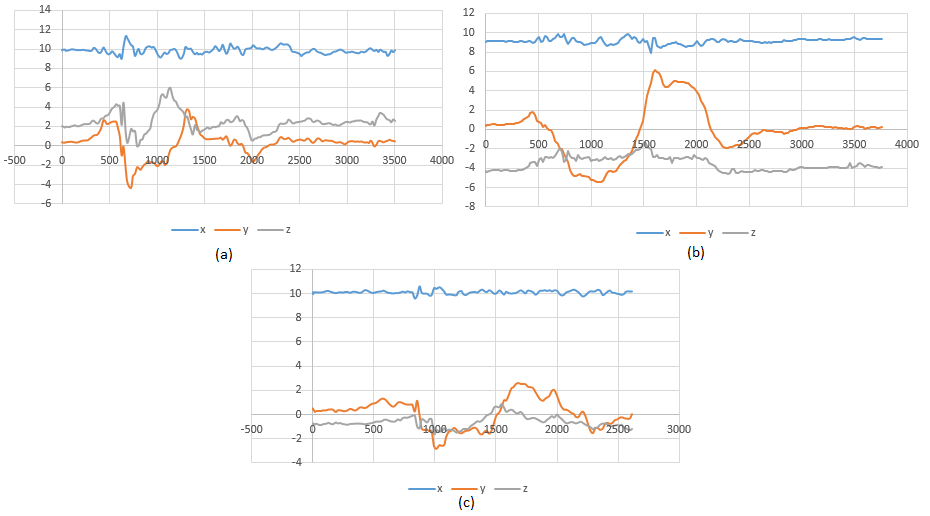
\includegraphics[scale=0.6]{Gambar/grafik-sensor-accelerometer-menggeleng.png}
\caption{Grafik nilai kuaternion dari sensor \textit{accelerometer} ketika pengguna menggeleng dengan posisi muka awal (a) menghadap ke depan, (b) menghadap ke atas, (c) menghadap ke kiri atas.} 
\label{fig:grafik-sensor-accelerometer-menggeleng}
\end{figure}

Gambar \ref{fig:grafik-sensor-accelerometer-menggeleng} merupakan grafik yang terbentuk dari nilai yang diterima oleh sensor \textit{accelerometer} ketika pengguna menggeleng. Pada grafik (a), nilai x konstan di sekitar angka 10. Nilai y dengan z pada grafik (a) menaik dan menurun ketika pengguna menggelengkan kepala. Pada grafik (b) nilai x terlihat konstan di sekitar nilai 10 dan nilai z sedikit tidak beraturan di sekitar nilai -4 hingga -2. Nilai y mengalami kenaikan dan penurunan saat menggeleng. Pada grafik (c) di Gambar \ref{fig:grafik-sensor-accelerometer-menggeleng} nilai x konstan di sekitar nilai 10. Nilai y menaik dan menurun, tetapi tidak beraturan. Nilai pada z juga mengalami sedikit kenaikan dan penurunan. Pada grafik (b) dengan (c) nilai z mengalami perubahan yang tidak beraturan dan puncak tertinggi dengan puncak terendahnya tidak terlalu berbeda jauh dengan nilai awalnya.

Dari keenam grafik tersebut terlihat bahwa nilai yang terpengaruh ketika pengguna sedang mengangguk adalah nilai x dengan z. Nilai y tidak berpengaruh karena nilai y cenderung konstan. Nilai yang terpengaruh ketika pengguna sedang menggeleng adalah nilai y. Nilai x terlihat konstan pada setiap grafik, tetapi nilai z mengalami sedikit pergerakan ketika pengguna sedang mengangguk sehingga tidak dapat dipastikan bahwa nilai z terpengaruh gerakan menggeleng. 

\subsection{Perekaman Grafik Sensor \textit{Gyroscope}}
\label{sec:analisis_grafik_sensor_gyroscope}
Perekaman menggunakan sensor \textit{gyroscope} menghasilkan percepatan angular yang terjadi setiap waktunya. Berbeda dengan sensor \textit{accelerometer} yang dapat terpengaruh oleh lingkungan sekitar seperti gravitasi dan percepatan lainnya, sensor ini hanya merekam perputaran yang terjadi pada perangkat saja. Hal ini sangat menguntungkan dalam mendeteksi suatu gerakan karena tidak harus memedulikan kasus dari pengaruh luar. 


\begin{figure}[htbp]
\centering
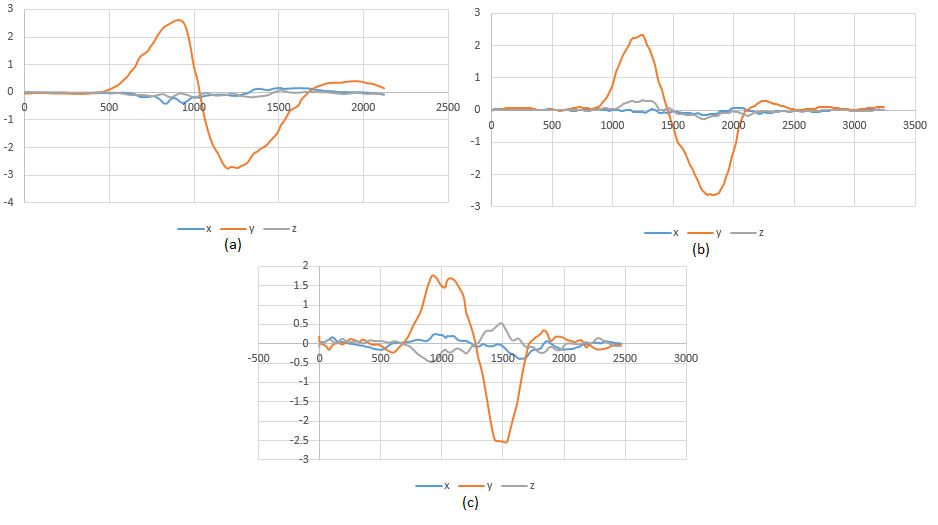
\includegraphics[scale=0.6]{Gambar/grafik-sensor-gyroscope-mengangguk.png}
\caption{Gambar grafik nilai sensor \textit{gyroscope} ketika pengguna mengangguk dengan posisi muka awal (a) menghadap ke depan, (b) menghadap ke atas, (c) menghadap ke kiri atas.}
\label{fig:grafik-sensor-gyroscope-mengangguk}
\end{figure}
Gambar \ref{fig:grafik-sensor-gyroscope-mengangguk} menunjukkan nilai-nilai sensor \textit{gyroscope} ketika pengguna sedang mengangguk. Grafik (a) membentuk sebuah \textit{hill} dan \textit{valley} pada nilai y. \textit{Hill} yang terjadi menunjukkan ketika pengguna menggerakkan kepalanya ke bawah, dan ketika kepala pengguna kembali ke posisi semula percepatan angularnya berbalik arah sehingga menimbulkan \textit{valley}. Nilai x dengan z cenderung bernilai 0. Grafik (b) mirip seperti grafik pada Gambar \ref{fig:grafik-sensor-gyroscope-mengangguk}. Begitu pula pada grafik (c) yang memiliki pola yang serupa dengan yang grafik-grafik sebelumnya.

\begin{figure}[htbp]
\centering
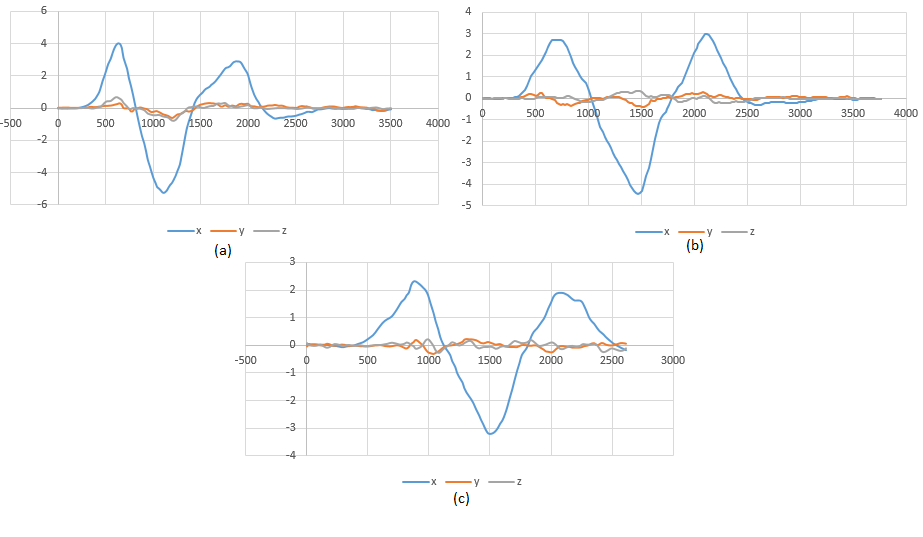
\includegraphics[scale=0.6]{Gambar/grafik-sensor-gyroscope-menggeleng.png}
\caption{Gambar grafik nilai sensor \textit{gyroscope} ketika pengguna menggeleng dengan posisi muka awal (a) menghadap ke depan, (b) menghadap ke atas, (c) menghadap ke kiri atas.} 
\label{fig:grafik-sensor-gyroscope-menggeleng}
\end{figure}

Gambar \ref{fig:grafik-sensor-gyroscope-menggeleng} menunjukkan nilai-nilai sensor \textit{gyroscope} ketika pengguna sedang menggeleng. Pada grafik (a) nilai yang mengalami kenaikan dan penurunan adalah nilai x dan nilai-nilai lainnya cenderung berada pada nilai 0. Nilai x membentuk 2 buah \textit{hill} dan 1 buah \textit{valley}. \textit{Hill} pertama terjadi ketika pengguna menggerakkan kepalanya ke kiri. \textit{Valley} pertama terjadi ketika pengguna menggerakkan kepalanya ke kanan. \textit{Hill} kedua terjadi ketika pengguna menggerakkan kepalanya kembali ke posisi semula. Pada grafik (b) dengan grafik (c) menunjukkan pola grafik yang serupa dengan grafik pada Gambar (a).

Dari hasil-hasil tersebut dapat disimpulkan bahwa arah pandang pengguna tidak memengaruhi sensor \textit{gyroscope} dalam mendeteksi gerakan kepala. Nilai-nilai yang dikembalikan oleh sensor \textit{gyroscope} memiliki  pola grafik yang jauh lebih rapi dibandingkan grafik-grafik yang dihasilkan oleh sensor \textit{accelerometer}. Selain itu sensor gyroscope hanya menggunakan 1 jenis nilai yang dipengaruhi oleh pergerakan kepala, sedangkan accelerometer ada 2 jenis nilai yang dipengaruhi gerakan kepala pada saat mengangguk. Oleh karena itu sensor gryoscope lebih baik dalam mendeteksi gerakan yang terjadi pada perangkat android.

\subsection{Perekaman Grafik Sensor \textit{Rotation Vector}}
\label{sec:analisis_grafik_sensor_rotation_vector}

Perekaman menggunakan sensor \textit{rotation vector} menghasilkan sebuah kuaternion yang merupakan representasi perputaran yang terjadi pada perangkat Android. Perputaran ini diartikan dengan suatu vektor sebagai sumbu putarnya dan sudut perputarannya. Berbeda dengan sensor \textit{gyroscope} yang merekam kecepatan perputaran yang terjadi pada suatu waktu, sensor \textit{rotation vector} mengembalikan nilai kuaternion untuk mendefinisikan suatu kondisi putaran pada saat itu. 

\begin{figure}[htbp]
\centering
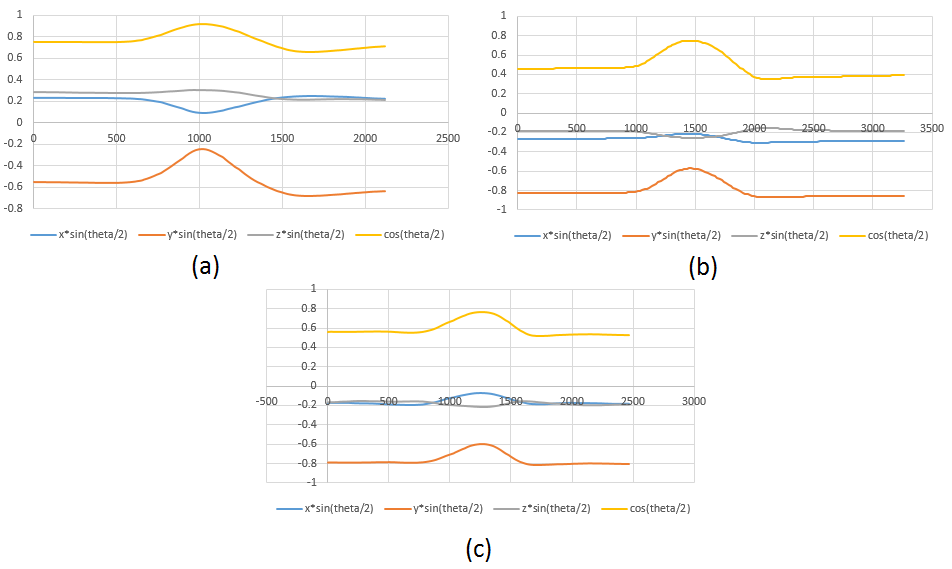
\includegraphics[scale=0.6]{Gambar/grafik-sensor-rot-vector-mengangguk.png}
\caption{Grafik nilai kuaternion dari sensor \textit{rotation vector} ketika pengguna mengangguk dengan posisi muka awal (a) menghadap ke depan, (b) menghadap ke atas, (c) menghadap ke kiri atas.} 
\label{fig:grafik-sensor-rot-vector-mengangguk}
\end{figure}

Gambar \ref{fig:grafik-sensor-rot-vector-mengangguk} menunjukkan nilai-nilai sensor \textit{rotation vector} ketika pengguna sedang mengangguk. Pada grafik (a) terbentuk sebuah \textit{hill} pada garis berwarna jingga dengan kuning, dan \textit{valley} pada garis berwarna biru. Garis yang berwarna abu cenderung stabil di angka 0.3. Grafik (b) menunjukkan pola yang mirip pada bagian (a) namun berbeda nilainya saja. Pada grafik (a) garis berwarna kuning dimulai pada angka sekitar 0.7, sedangkan pada grafik (b) garis berwarna jingga dimulai pada angka sekitar 0.4. Garis biru pada grafik ini tidak membentuk sebuah \textit{valley} seperti  pada grafik pada grafik (a). Garis berwarna abu cenderung konstan pada nilai -0.2, sedangkan pada grafik (a) cenderung konstan di sekitar 0.3. Garis berwarna jingga memiliki pola yang sama dengan garis berwarna kuning, hanya berbeda pada nilainya saja. Seperti pada grafik-grafik sebelumnya, grafik (c) ini memiliki pola yang sama dengan grafik lainnya. Grafik ini juga hanya nilainya saja yang berbeda dengan grafik lainnya. Kemiripan pola ini memungkinkan mempermudah pendeteksian gerakan kepala. 

\begin{figure}[htbp]
\centering
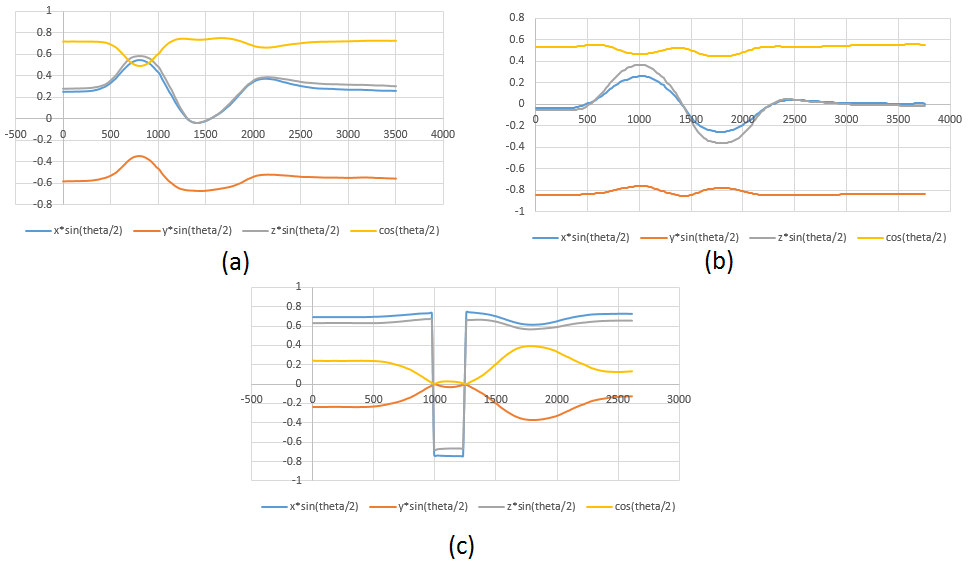
\includegraphics[scale=0.6]{Gambar/grafik-sensor-rot-vector-menggeleng.png}
\caption{Grafik nilai kuaternion dari sensor \textit{rotation vector} ketika pengguna menggeleng dengan posisi muka awal (a) menghadap ke depan, (b) menghadap ke atas, (c) menghadap ke kiri atas.} 
\label{fig:grafik-sensor-rot-vector-menggeleng}
\end{figure}

Gambar \ref{fig:grafik-sensor-rot-vector-menggeleng} menunjukkan nilai-nilai sensor \textit{rotation vector} ketika pengguna sedang menggeleng. Pada grafik (a) terbentuk sebuh \textit{hill} yang diikuti dengan \textit{valley} pada garis berwarna biru dengan abu-abu. Garis berwarna kuning membentuk suatu \textit{valley} yang setelahnya cenderung konstan. Berbeda pada garis kuning yang membentuk \textit{hill} kemudian setelahnya cenderung konstan. Grafik (b) memiliki kemiripan dengan grafik (a), garis biru dengan garis abu-abu memiliki pola yang sama yaitu membentuk \textit{hill} dengan \textit{valley} ketika pengguna menggelengkan kepala. Garis kuning dengan jingga cenderung konstan, berbeda dengan grafik (a) yang membentuk \textit{hill} atau \textit{valley}. Pada grafik (c) garis-garis membentuk suatu pola yang tidak normal. Garis kuning membentuk sebuah \textit{valley}, tetapi membentuk suatu \textit{hill} kecil ketika nilainya mencapai nilai 0 pada mili detik ke 1000. Garis jingga memiliki pola yang berlawanan dengan garis kuning. Pada saat garis kuning dengan garis jingga mencapai angka 0 perubahan drastis pun terjadi pada garis biru dengan abu-abu. Pada mili detik ke 1000 garis biru dengan abu mengalami perubahan nilai yang sangat drastis. Kedua nilai tersebut berubah dari nilai yang berkisar diantara 0.6 sampai 0.7 menjadi berkisar diantara -0.7 sampai -0.8. Kasus ini tidak berarti sensor sedang mengalami kegagalan akurasi (\textit{accuracy fail}), tetapi memang seperti itulah karakteristik dari perputaran menggunakan kuaternion pada android. Perputaran yang terjadi pada batas mendekati sebelum terjadinya dengan setelah perubahan nilai yang drastis memiliki hasil perputaran yang sama. Hal ini disebabkan karena melakukan perputaran dengan vektor sebagai sumbu dapat memiliki 2 buah nilai yang sejenis. Dua buah nilai tersebut menghasilkan perputaran yang sama ketika arah vektor dengan arah putarnya dibalikkan seperti yang ditunjukkan pada Gambar \ref{fig:penjelasan-perputaran-quaternion-android-sensor}. Sepertinya pada sistem android nilai $\cos (theta/2)$ didesain agar tidak bernilai negatif, sehingga nilai-nilai yang lainnya mengalami perubahan nilai yang drastis ketika nilai $\cos (theta/2)$ mencapai angka 0.


\begin{figure}[htbp]
\centering
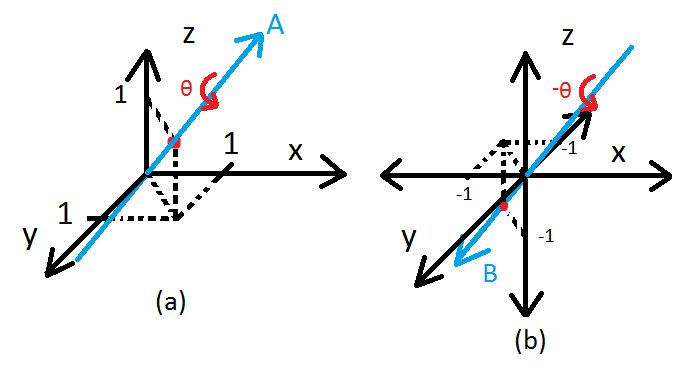
\includegraphics[scale=0.6]{Gambar/penjelasan-perputaran-quaternion-android-sensor.png}
\caption{Dua buah rotasi yang identik dengan nilai kuaternion yang berbeda.} 
\label{fig:penjelasan-perputaran-quaternion-android-sensor}
\end{figure}

\section{Analisis Data Sensor untuk Mendeteksi Gerakan Kepala}

Dari ketiga hasil percobaan pada sensor-sensor pada Bab \ref{sec:perekaman_data_sensor} dapat disimpulkan bahwa sensor \textit{gyroscope} adalah sensor yang terbaik untuk mendeteksi gerakan kepala. Data dari sensor \textit{accelerometer} sulit untuk digunakan dalam mendeteksi gerakan kepala karena terganggu dengan aktivitas-aktivitas di luar gerakan pengguna yang juga ikut terekam oleh sensor \textit{accelerometer}. Data dari sensor \textit{rotation vector} juga lebih rumit dibandingkan sensor \textit{gyroscope}. Hal ini karena perputaran yang direkam oleh sensor \textit{rotation vector} merekam kondisi putar pada suatu saat. Hasil rekaman ini mempersulit pada saat pendeteksian gerakan kepala karena harus melakukan proses untuk menghitung kecepatan kepala bergerak, agar dapat membedakan gerakan mengangguk atau menggeleng atau hanya menoleh biasa. 
Dalam mendeteksi gerakan mengangguk dengan menggeleng banyak batas-batas yang perlu diperhatikan. Batas-batas tersebut untuk mengetahui apakah pengguna benar-benar mengangguk atau menggeleng atau hanya menoleh biasa. Batas-batas yang perlu diperhatikan adalah:

\begin{itemize}
	\item Kecepatan pengguna menoleh.
	\item Selang waktu antara gerakan kepala pengguna yang berlawanan.
	\item Simpangan terbesar kepala saat mengangguk atau menggeleng.
\end{itemize}

Kecepatan pengguna menjadi batas karena gerakan kepala yang kecepatannya cenderung pelan biasanya bukan merupakan gerakan mengangguk atau pun menggeleng. Kecepatan ini dapat langsung diperoleh menggunakan sensor \textit{gyroscope}. Kecepatan yang dibutuhkan adalah kecepatan perputaran maksimum yang dilakukan oleh pengguna. Kecepatan maksimum dapat diperoleh dengan mengambil nilai puncak tertinggi dengan terendah. Jika nilai puncaknya mencapai kecepatan tertentu, gerakan tersebut dapat diperkirakan merupakan gerakan mengangguk atau pun menggeleng.

Gerakan menggeleng atau mengangguk biasanya memiliki selang waktu yang sangat sempit, karena pengguna biasanya langsung melawan arah gerakan kepala secara langsung ketika sedang mengangguk atau pun menggeleng. Nilai ini dapat diperoleh dengan menghitung jarak antara \textit{hill} dengan \textit{valley} yang terbentuk pada grafik seperti yang dijelaskan pada Gambar \ref{fig:grafik-penjelasan-jarak-waktu-melawan-gerakan} dan Gambar \ref{fig:grafik-penjelasan-jarak-waktu-melawan-gerakan-mengangguk}. Idealnya gerakan menggeleng tidak memiliki rentang waktu ini, namun mungkin sebagian orang masih menghasilkan rentang waktu yang cukup sedikit. Oleh karena itu mungkin batas waktu yang ditentukan di sini adalah sekitar 100 milidetik. Jika rentang waktunya melebihi batas waktu tersebut, maka gerakan tersebut mungkin bukan merupakan gerakan mengangguk atau pun gerakan menggeleng. 

\begin{figure}[htbp]
\centering
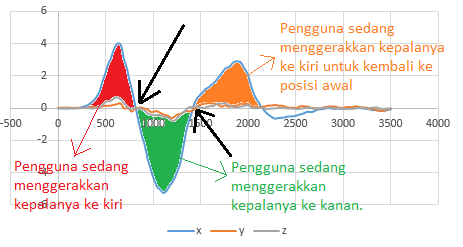
\includegraphics[scale=0.6]{Gambar/grafik-penjelasan-jarak-waktu-melawan-gerakan.png}
\caption{Grafik pada saat pengguna menggeleng.} 
\label{fig:grafik-penjelasan-jarak-waktu-melawan-gerakan}
\end{figure}

\begin{figure}[htbp]
\centering
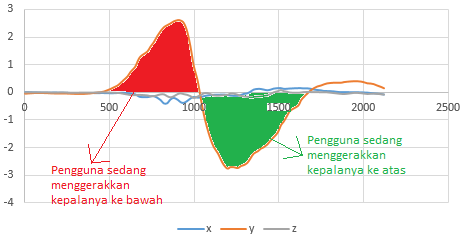
\includegraphics[scale=0.6]{Gambar/grafik-penjelasan-jarak-waktu-melawan-gerakan-mengangguk.png}
\caption{Grafik pada saat pengguna mengangguk.} 
\label{fig:grafik-penjelasan-jarak-waktu-melawan-gerakan-mengangguk}
\end{figure}

Simpangan terbesar ini juga penting untuk dijadikan batasan-batasan dalam mendeteksi gerakan mengangguk atau pun menggeleng. Simpangan kepala yang sangat kecil dapat diragukan untuk dianggap sebagai gerakan mengangguk atau menggeleng. Simpangan ini dapat diperoleh dengan menghitung luas yang dibentuk dari \textit{hill} atau \textit{valley} yang terbentuk pada grafik. Contoh pada Gambar \ref{fig:grafik-penjelasan-jarak-waktu-melawan-gerakan} simpangan terbesar yang terjadi ketika pengguna menggerakkan kepalanya pertama kali ke kiri adalah luas pada bidang yang diarsir merah. Simpangan terbesar yang terjadi ketika pengguna menggerakkan kepalanya ke kanan adalah luas bidang yang di-arsir berwarna hijau. Contoh pada Gambar \ref{fig:grafik-penjelasan-jarak-waktu-melawan-gerakan-mengangguk} simpangan terbesar yang terjadi ketika pengguna menggerakkan kepalanya ke atas adalah luas pada bidang yang diarsir merah.

\section{Analisis Metode Pendeteksian Gerakan Kepala}
\label{sec:analisis_metode_pendeteksi_gerakan_kepala}

Seperti yang sudah dijelaskan pada bab \ref{sec:android_sensor_framework}, data didapatkan setiap ada perubahan nilai pada sensor dengan rentang waktu tertentu, bergantung dengan konfigurasinya. Pendeteksian ini membutuhkan data yang \textit{real-time}, sehingga lebih baik jika menggunakan konfigurasi kecepatan pengambilan data setiap 20 mikro detik. Penggunaan konfigurasi dengan kecepatan 0 mikro detik tidak terlalu baik, karena menggunakan kemampuan processor yang sangat tinggi.

\subsection{Algoritma Mendeteksi Gerakan Mengangguk}
\label{ssec:algoritma_mendeteksi_gerakan_mengangguk}

Algoritma dipanggil setiap kali ada perubahan nilai dari sensor. Algoritma ini menyimpan nilai-nilai batas-batas yang telah ditentukan, luas yang terbentuk, nilai tertinggi, waktu mulai, dan waktu akhir dari suatu \textit{hill} atau \textit{valley}. Algoritma ini dipanggil secara berulang-ulang hingga data yang dikumpulkan dapat menghasilkan suatu kesimpulan mengangguk. Data disimpan pada atribut, agar setiap pemanggilan dapat melanjutkan dari pemanggilan sebelumnya. 

Berikut adalah keterangan dari data-data yang disimpan pada atribut:
\begin{itemize}
	\item \texttt{currPassLimitUp}, atribut ini menunjukkan bahwa pada saat ini gerakan pengguna sedang bergerak ke atas dan melebihi batas kecepatan sudutnya.
	\item \texttt{currPassLimitDown}, atribut ini menunjukkan bahwa pada saat ini gerakan pengguna sedang bergerak ke bawah dan melebihi batas kecepatan sudutnya.
	\item \texttt{angSpeedLimit}, atribut ini menyimpan batas kecepatan sudut.
	\item \texttt{lastYAngSpeed}, atribut ini memiliki kecepatan sudut Y pada pemanggillan method sebelumnya. 
	\item \texttt{lastT}, atribut ini memiliki waktu dipanggilnya method sebelumnya. 
	\item \texttt{calcArea}, atribut ini menyimpan besar luas \textit{hill} atau, \textit{valley} yang terjadi. Luas \textit{hill} bernilai positif, dan nilai \textit{valley} bernilai negatif. 
	\item \texttt{startTValley}, atribut ini menyimpan waktu mulai \textit{valley} yang memenuhi syarat kecepatan sudut minimal. 
	\item \texttt{endTValley}, atribut ini menyimpan waktu akhir \textit{valley} yang memenuhi syarat kecepatan sudut minimal.
	\item \texttt{startTCurrMotion}, atribut ini menyimpan waktu mulai suatu gerakan(\textit{hill} atau \textit{valley}) yang sedang berlangsung sekarang.
	\item \texttt{endTCurrMotion}, atribut ini menyimpan waktu akhir suatu gerakan(\textit{hill} atau \textit{valley}) yang sedang berlangsung sekarang.
	\item \texttt{deviationLimit} adalah batas simpangan untuk melakukan gerakan mengangguk.
	\item \texttt{deviationMotionDown}, atribut ini menyimpan simpangan yang terjadi ketika pengguna menggeraka kepalanya ke bawah. 
	\item \texttt{deviationMotioUp}, atribut ini menyimpan simpangan yang terjadi ketika pengguna menggeraka kepalanya ke atas. 
\end{itemize}
\begin{algorithm}
	\caption{Nod Detection Algoritm}
	\label{alg:algoritma-pendeteksi-gerakan-mengangguk}
	\begin{algorithmic}[1]
	\Function{detectNod}{$yAngSpeed$}
		\State $currT \gets $current Time 
		\If {$yAngSpeed > angSpeedLimit$}
			\State $currPassLimitUp \gets true$
		\ElsIf {$yAngSpeed < angSpeedLimit * -1$}
			\State $currPassLimitDown \gets true$
		\EndIf
		\If {X values intersect with x(time) axis}
			\State $xIntersect \gets ((-lastYAngSpeed / (yAngSpeed - lastYAngSpeed)) * (currT - lastT))+lastT$
			\State $endTCurrMotion \gets xIntersect$
			\State $areaBeforeIntersect \gets ((xIntersect - lastT) / 1000) * lastYAngSpeed / 2$
			\State $calcArea \gets calcArea + areaBeforeIntersect$
			\If {$currPassLimitDown$}
				\State $startTValley \gets startTCurrMotion$
				\State $endTValley \gets endTCurrMotion$
				\State $deviationMotionDown \gets calcArea$
				\If {$deviationMotionDown < deviationLimit * -1$}
					\State $passLimitDownDeviation \gets true$
				\EndIf
			\ElsIf {$currPassLimitUp$}
				\State $startTHill \gets startTCurrMotion$
				\State $endTHill \gets endTCurrMotion$
				\State $deviationMotionUp \gets calcArea$
				\If {$deviationMotionUp > deviationLimit$}
					\State $passLimitUpDeviation \gets true$
				\EndIf
			\EndIf
			\State $calcArea \gets 0$
			\State $areaAfterIntersect \gets ((currT - xIntersect) / 1000) * yAngSpeed / 2$ 
			\State $calcArea \gets calcArea + areaAfterIntersect$ 
			\State $startTCurrMotion \gets xIntersect$ 
			\State $currPassLimitDown \gets false$ 
			\State $currPassLimitUp \gets false$ 
		\Else 
			\State $calcArea \gets calcArea + ((lastYAngSpeed + yAngSpeed) / 1000) * (currT - lastT) / 2$
		\EndIf
		\State $lastYAngSpeed \gets yAngSpeed$
		\State $lastT \gets currT$
		
		\If {hill and valley time values has been set \textbf{AND} all condition have been met}
			\Return $true$
		\Else {
			\Return $false$}
		\EndIf
	\EndFunction  
	\end{algorithmic}
\end{algorithm}

Algoritma \ref{alg:algoritma-pendeteksi-gerakan-mengangguk} mengembalikan nilai true jika pengguna sedang mengangguk. Baris ke-2 hingga baris ke-8 adalah untuk mengecek kecepatan putar sekarang, apakah sudah melampaui batas yang ditentukan atau belum. Untuk mengetahui titik potong secara akurat dapat menggunakan rumus persamaan garis dari dua buah titik yang dinotasikan dengan Notasi \ref{eq:persamaan-garis-dua-titik}.   

\begin{equation}
		\frac{y-y_1}{y_2-y_1} = \frac{x-x_1}{x_2-x_1} \\
\label{eq:persamaan-garis-dua-titik}
\end{equation}
dengan,
\[
	\begin{split}
		y_1 = & lastYAngSpeed\\
		y_2 = & yAngSpeed\\
		x_1 = & lastT\\
		x_2 = & currT
	\end{split}
\]

Notasi \ref{eq:persamaan-garis-dua-titik} dijabarkan sesuai dengan penjabaran \ref{eq:aljabar-pencarian-titik-potong} sehingga menjadi rumus yang berada pada algoritma \ref{alg:algoritma-pendeteksi-gerakan-mengangguk} baris ke-10. Nilai titik potong x ini juga menjadi indikator waktu untuk rentang waktu dari suatu \textit{hill} atau \textit{valley}, yang digunakan untuk mendapatkan jarak waktu pada saat pengguna melawan arah gerakan. Baris ke-14 hingga ke-25 pada algoritma \ref{alg:algoritma-pendeteksi-gerakan-mengangguk} adalah untuk mengecek apakah simpangan yang terjadinya sudah melewati batas yang ditetapkan atau belum dan mencatatnya ke dalam atribut \texttt{passLimitDownDeviation} atau \texttt{passLimitUpDeviation}. Pada baris ke-26 hingga ke-28 untuk memulai menghitung luas yang baru. Baris ke-32 dan baris ke-33 untuk menghitung luas ketika tidak berpotongan dengan sumbu x. Baris ke-36 untuk pengecekan jarak antara \textit{hill} dengan \textit{valley} dapat diselesaikan dengan mengurangi waktu mulai \textit{hill} dengan waktu akhir \textit{valley}. Sehingga hasil untuk mengecek apakah semua batas sudah terpenuhi dapat diselesaikan dengan operasi (AND) biasa. 

\begin{equation}
	\begin{split}
		y = & 0\\		
		\frac{0-y_1}{y_2-y_1} = & \frac{x-x_1}{x_2-x_1} \\
		\frac{-y_1}{y_2-y_1} (x_2-x_1) = & x-x_1 \\
		x = & (\frac{-y_1}{y_2-y_1} (x_2-x_1)) +x_1
	\end{split}
\label{eq:aljabar-pencarian-titik-potong}
\end{equation}


\subsection{Algoritma Mendeteksi Gerakan Menggeleng}
\label{ssec:algoritma_mendeteksi_gerakan_menggeleng}

Sama seperti pada pendeteksian gerakan mengangguk, algoritma ini dipanggil setiap kali ada perubahan nilai sensor. Algoritma ini juga menyimpan batas-batas, waktu mulai dan berakhirnya suatu \textit{hill} atau \textit{valley}. Algoritma ini dipanggil setiap ada perubahan nilai sensor dan data-data yang diperoleh disimpan pada atribut. Algoritma ini juga dipanggil secara berulang-ulang hingga data yang dikumpulkan dapat menghasilkan suatu kesimpulan menggeleng.

Sebagian atribut memiliki kegunaan yang sama dengan algoritma pendeteksian gerakan mengangguk. Berikut adalah keterangan dari data-data yang disimpan pada atribut yang belum dijelaskan pada algoritma pendeteksian gerakan mengangguk:
\begin{itemize}
	\item \texttt{currPassLimitLeft}, atribut ini menunjukkan bahwa pada saat ini gerakan pengguna sedang bergerak ke kiri dan melebihi batas kecepatan sudutnya.
	\item \texttt{currPassLimitRight}, atribut ini menunjukkan bahwa pada saat ini gerakan pengguna sedang bergerak ke kanan dan melebihi batas kecepatan sudutnya.
	\item \texttt{lastXAngSpeed}, atribut ini memiliki kecepatan sudut X pada pemanggillan method sebelumnya. 
	\item \texttt{deviationMotionLeft}, atribut ini menyimpan simpangan yang terjadi ketika pengguna menggeraka kepalanya ke kiri. 
	\item \texttt{deviationMotioRight}, atribut ini menyimpan simpangan yang terjadi ketika pengguna menggeraka kepalanya ke kanan. 
\end{itemize}


\begin{algorithm}
	\caption{Shook Detection Algoritm}
	\label{alg:algoritma-pendeteksi-gerakan-menggeleng}
	\begin{algorithmic}[1]
	\Function{detectShook}{$xAngSpeed$}
		\State $currT \gets $current Time
		\If {$xAngSpeed > angSpeedLimit$}
			\State $currPassLimitLeft \gets true$
		\ElsIf {$xAngSpeed < angSpeedLimit * -1$}
			\State $currPassLimitRight \gets true$
		\EndIf
		\If {X values intersect with x(time) axis}
			\State $xIntersect \gets ((-lastXAngSpeed / (xAngSpeed - lastXAngSpeed)) * (currT - lastT))+lastT$
			\State $endTCurrMotion \gets xIntersect$
			\State $areaBeforeIntersect \gets ((xIntersect - lastT) / 1000) * lastXAngSpeed / 2$
			\State $calcArea \gets calcArea + areaBeforeIntersect$
			\If {$currPassLimitRight$}
				\State $deviationMotionRight \gets calcArea$
				\If {$deviationMotionRight < deviationLimit$}
					\State $valleyTimes.add($start and end time valley$)$
				\EndIf
			\ElsIf {$currPassLimitLeft$}
				\State $deviationMotionUp \gets calcArea$
				\If {$deviationMotionUp > deviationLimit * -1$}
					\State $hillTimes.add($start and end time hill$)$
				\EndIf
			\EndIf
			\State $calcArea \gets 0$
			\State $areaAfterIntersect \gets ((currT - xIntersect) / 1000) * xAngSpeed / 2$ 
			\State $calcArea \gets calcArea + areaAfterIntersect$ 
			\State $startTCurrMotion \gets xIntersect$ 
			\State $currPassLimitRight \gets false$ 
			\State $currPassLimitLeft \gets false$ 
		\Else 
			\State $calcArea \gets calcArea + ((lastXAngSpeed + xAngSpeed) / 1000) * (currT - lastT) / 2$
		\EndIf
		\State $lastXAngSpeed \gets xAngSpeed$
		\State $lastT \gets currT$
		\If {head moves right first \textbf{AND} time range between hill and valley no exceed the limit.}
			\Return $true$ 
		\ElsIf {head moves left first \textbf{AND} time range between hill and valley no exceed the limit.}
			 \Return $true$
		\Else {
			 \Return $false$}
		\EndIf
	\EndFunction  
	\end{algorithmic}
\end{algorithm} 

Sebagian besar algoritma untuk mendeteksi gerakan menggeleng memiliki kemiripan dengan algoritma untuk mendeteksi gerakan mengangguk. Pada algoritma menggeleng data waktu mulai dan berakhirnya suatu \textit{hill} atau \textit{valley} disimpan pada atribut dengan tipe data \textit{List}. Atribut-atribut yang menggunakan tipe data \textit{List} ini adalah \texttt{valleyTimes} dan \texttt{hillTimes}. Data-data waktu terjadinya bukti atau \textit{valley} yang dimasukkan ke dalam \textit{List} ini diartikan sudah memenuhi syarat dari batas-batas simpangan dan kecepatan sudutnya. \texttt{List} ini dikosongkan kembali jika salah satu \textit{List}-nya sudah lebih dari dua atau kedua \textit{List} tersebut sudah memiliki isi sebanyak dua, atau lebih. 

Untuk pengecekan jarak waktu antara \textit{valley} dengan \textit{hill} dilakukan sebanyak dua kali. Pengecekan pertama yaitu untuk pengecekan jarak waktu antara \textit{valley} atau \textit{hill} pertama dengan kedua. Pengecekan kedua yaitu untuk pengecekan jarak waktu antara \textit{valley} atau \textit{hill} kedua dengan ketiga. Perhitungan jarak waktu antara \textit{valley} atau \textit{hill} pertama dengan kedua dapat dilakukan dengan mengurangi waktu dimulainya \textit{valley} atau \textit{hill} kedua dengan waktu berakhirnya \textit{valley} atau \textit{hill} pertama. Begitu pula dengan perhitungan jarak waktu antara \textit{valley} atau \textit{hill} kedua dengan ketiga.



\section{Analisis Aplikasi Permainan dengan Algoritma Deteksi Gerakan Kepala}
\label{sec:analisis_aplikasi_permainan_dengan_algoritma_deteksi_gerakan_kepala}

Pada skripsi ini dibuat suatu aplikasi yang mengimplementasikan algoritma deteksi gerakan kepala. Aplikasi ini merupakan suatu permainan dengan menggunakan gerakan kepala sebagai salah satu masukkan pada permainan ini. Masukkan dari gerakan kepala hanyalah mengangguk dan menggeleng. Masukkan ini hanya dapat digunakan ketika aplikasi membutuhkan jawaban dialog yang hanya dapat dijawab dengan ya atau tidak saja. Oleh karena itu permainan ini menggunakan pertanyaan dialog sebagai inti dari permainannya.

Aplikasi ini memiliki beberapa fungsi yang dimiliki. Fungsi utama dalam permainan ini yaitu dengan menggunakan anggukan dan gelengan sebagai masukan pada permainan. Fungsi-fungsi lainnya pada permainan ini dijelaskan dengan menggunakan diagram \textit{use case} pada Gambar \ref{fig:use_case_diagram} dan skenario pada Tabel \ref{tab:tabel_skenario_memulai_permainan} hingga Tabel \ref{tab:tabel_skenario_memulai_permainan}.


\begin{figure}[htbp]
\centering
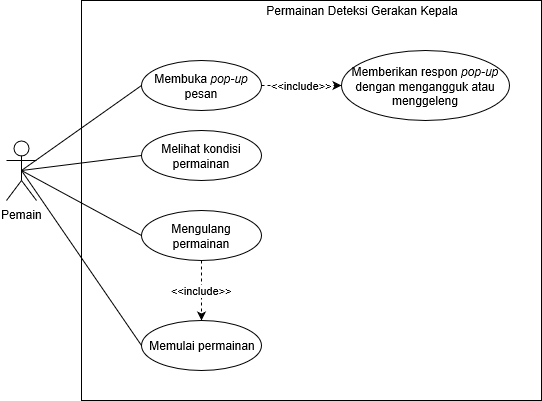
\includegraphics[scale=0.6]{Gambar/usecasediagram.png}
\caption{Diagram \textit{use case} aplikasi permainan deteksi gerakan kepala}
\label{fig:use_case_diagram}
\end{figure}


\begin{table}[]
    \centering
    \begin{tabular}{|p{3cm}|p{10cm}|}
    \hline
        Nama & Memulai Permainan\\
    \hline
    \hline
        Deskripsi & Memulai permainan dari kondisi awal\\
    \hline
        Aktor & Pemain \\
    \hline
        Pre-kondisi & Aplikasi dimulai \\
    \hline
        Alur Skenario Utama & 
        \begin{enumerate}
            \item Sistem memuat aplikasi.
            \item Sistem memulai permainan.
        \end{enumerate}\\
    \hline
    \end{tabular}
    \caption{Tabel skenario memulai permainan.}
    \label{tab:tabel_skenario_memulai_permainan}
\end{table}


\begin{table}[]
    \centering
    \begin{tabular}{|p{3cm}|p{10cm}|}
    \hline
        Nama & Membuka \textit{pop-up} pesan\\
    \hline
    \hline
        Deskripsi & Memunculkan pesan berupa \textit{pop-up} pada pengguna dalam VR\\
    \hline
        Aktor & Pemain \\
    \hline
        Alur Skenario Utama & 
        \begin{enumerate}
            \item Pengguna melihat notifikasi baru yang dimunculkan oleh sistem.
            \item Pengguna mengklik notifikasi.
            \item Sistem memunculkan \textit{pop-up} pesan.
        \end{enumerate}\\
    \hline
    \end{tabular}
    \caption{Tabel skenario membuka \textit{pop-up} pesan.}
    \label{tab:tabel_skenario_membuka_pop-up_pesan}
\end{table}


\begin{table}[]
    \centering
    \begin{tabular}{|p{3cm}|p{10cm}|}
    \hline
        Nama & Memberikan respons \textit{pop-up} dengan menggeleng atau mengangguk\\
    \hline
    \hline
        Deskripsi & Memberikan jawaban terhadap pesan di \textit{pop-up} yang diberikan dengan menggunakan gerakan kepala, yaitu mengangguk dan menggeleng.\\
    \hline
        Aktor & Pemain \\
    \hline
        Pre-kondisi & \textit{Pop-up} telah muncul. \\
    \hline
        Alur Skenario Utama & 
        \begin{enumerate}
            \item Pengguna membaca pesan \textit{pop-up} yang telah muncul.
            \item Pengguna memberikan respons dengan mengangguk.
            \item Pesan pada \textit{pop-up} diubah menjadi "\textit{yes}".
        \end{enumerate}\\
    \hline
        Alur Skenario Alternatif & 
        \begin{enumerate}
            \item [2a.] Pengguna memberikan respons dengan menggeleng.
            \item [3a.] Pesan pada \textit{pop-up} diubah menjadi "\textit{no}".
        \end{enumerate}\\
    \hline
    \end{tabular}
    \caption{Tabel skenario memberikan respons \textit{pop-up} dengan menggeleng atau mengangguk.}
    \label{tab:tabel_skenario_memberikan_respons_pop-up_dengan_menggeleng_atau_mengangguk}
\end{table}


\begin{table}[]
    \centering
    \begin{tabular}{|p{3cm}|p{10cm}|}
    \hline
        Nama & Melihat kondisi permainan\\
    \hline
    \hline
        Deskripsi & Melihat status kondisi permainan.\\
    \hline
        Aktor & Pemain \\
    \hline
        Alur Skenario Utama & 
        \begin{enumerate}
            \item Pengguna mengarahkan posisi kepala ke panel kondisi permainan.
            \item Panel kondisi berubah-ubah seiring pemain memainkan permainannya.
        \end{enumerate}\\
    \hline
    \end{tabular}
    \caption{Tabel skenario melihat kondisi permainan.}
    \label{tab:tabel_skenario_melihat_kondisi_permainan}
\end{table}

\begin{table}[]
    \centering
    \begin{tabular}{|p{3cm}|p{10cm}|}
    \hline
        Nama & Mengulang permainan\\
    \hline
    \hline
        Deskripsi & Mengulang permainan kembali ke kondisi awal ketika permainan telah usai.\\
    \hline
        Aktor & Pemain \\
    \hline
        Pre-kondisi & Permainan telah usai. \\
    \hline
        Alur Skenario Utama & 
        \begin{enumerate}
            \item Pengguna mengklik (Menarik pelatuk pada Google Cardboard).
            \item Mengulang permainan dari awal.
        \end{enumerate}\\
    \hline
    \end{tabular}
    \caption{Tabel skenario mengulang permainan.}
    \label{tab:tabel_skenario_mengulang_permainan}
\end{table}

Algoritma pendeteksi gerakan kepala pada subbab \ref{sec:analisis_aplikasi_permainan_dengan_algoritma_deteksi_gerakan_kepala} tidak memiliki desain kelas yang baik. Algoritma tersebut mengerjakan beberapa tugas berbeda dalam waktu yang sama, sehingga algoritma tersebut melanggar prinsip desain SOLID pertama yaitu Single Responsibility Principle. Sehingga perlu dibuat kelas-kelas baru untuk memisahkan tugas yang berbeda ke dalam suatu kelas baru tersebut. Oleh sebab itu perlu dibuat diagram kelas untuk menjelaskan kelas-kelas yang diperlukan. 

Pada subbab ini dibuat suatu diagram kelas sederhana untuk menjelaskan kelas-kelas yang dibutuhkan dalam membuat aplikasi permainan yang mengimplementasikan algoritma deteksi gerakan kepala. Aplikasi ini dibuat dengan menggunakan Game Engine Unity. Game Engine Unity menggunakan \textit{design pattern} MVC (Model-View-Controller) dalam pengimplementasiannya. Hal ini menyebabkan diagram kelas yang dibuat memiliki bentuk seperti \textit{design pattern} MVC. Meski diagram kelas yang dibuat memiliki bentuk MVC, namun diagram kelas ini tidak memiliki bagian \textit{view}-nya karena bagian view sudah diimplementasikan pada Game Engine Unity dengan mengunakan GameObject Hierarcy yang telah dijelaskan \ref{ssec:struktur_hierarki_gameobject}. Oleh karena itu diagram kelas ini hanya memiliki bagian \textit{controller} dan bagian \textit{model} saja. \textit{Package} "Head Motion Detector" merupakan bagian yang serupa dengan \textit{model} pada \textit{design pattern} MVC. Gambar \ref{fig:diagram_kelas_algoritma_pendeteksi_gerakan_kepala_sederhana} merupakan diagram kelas permainan yang menggunakan algoritma deteksi gerakan kepala.


\begin{figure}[htbp]
\centering
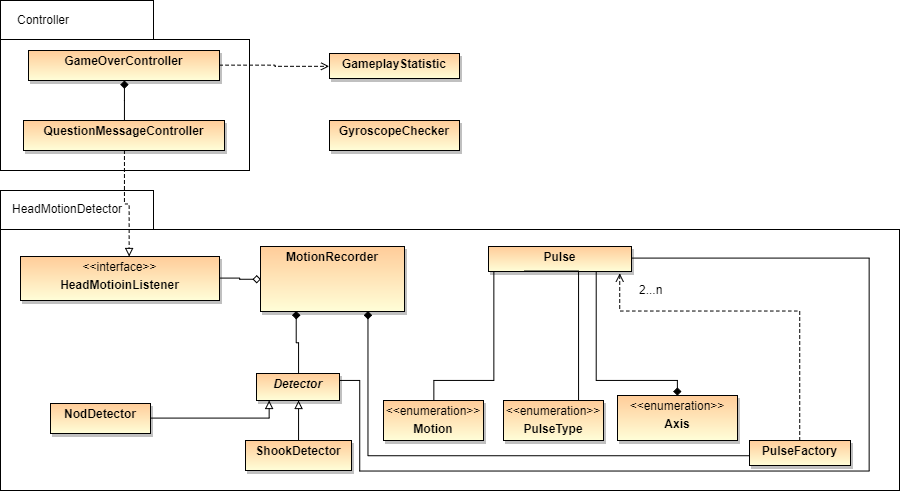
\includegraphics[scale=0.4]{Gambar/diagram-kelas-algoritma-pendeteksi-gerakan-kepala-sederhana.png}
\caption{\textit{Screenshot} task yang diberikan aplikasi InMind VR.}
\label{fig:diagram_kelas_algoritma_pendeteksi_gerakan_kepala_sederhana}
\end{figure}
Berikut ini adalah penjelasan dari kelas-kelas pada diagram di Gambar \ref{fig:diagram_kelas_algoritma_pendeteksi_gerakan_kepala_sederhana}.
\begin{itemize}
    \item Kelas GameplayStatistic\\
    Kelas ini bertujuan untuk menyimpan seluruh atribut-atribut statis pada keseluruhan permainan.
    \item Kelas GyroscopeChecker\\
    Kelas ini digunakan untuk mengecek apakah perangkat yang sedang menjalankan permainan ini memiliki sensor gyroscope.
    \item Package Controller
    \begin{itemize}
        \item Kelas GameOverController\\
        Kelas ini bertujuan untuk mendeteksi kondisi \textit{game over} dan menampilkan pesan \textit{game over}.
        \item Kelas QuestionMessageController\\
        Kelas ini digunakan untuk mengatur tampilan pesan pertanyaan pada permainan. 
    \end{itemize}
    \item Package HeadMotionDetector
    \begin{itemize}
        \item interface HeadMotionListener\\
        Interface ini di-\textit{implement} oleh kelas-kelas yang menggunakan hasil dari pendeteksian gerakan kepala.
        \item Kelas MotionRecorder\\
        Kelas ini digunakan untuk merekam, menentukan, dan mendeteksi gerakan kepala. 
        \item Kelas PulseFactory\\
        Kelas ini berguna untuk mendeteksi \textit{Pulse} yang terjadi pada grafik data gyroscope.
        \item Kelas Detector\\
        Kelas ini merupakan kelas yang mendefinisikan pendeteksi gerakan kepala. Sub-class kelas ini adalah NodDetector dengan ShookDetector
        \item Kelas NodDetector dengan ShookDetector\\
        Kelas ini berisi algoritma untuk mendeteksi gerakan mengangguk atau menggeleng. Kelas ini merupakan turunan dari kelas Detector
        \item Kelas Pulse\\
        Kelas ini digunakan hanya untuk menyimpan karakteristik-karakteristik dari suatu \textit{Pulse} yang terbentuk oleh kelas PulseDetector. 
    \end{itemize}
\end{itemize}